
\section{Architettura di HBS}

L'architettura fisica di HBS si integra nell'architettura fisica dell'istituto bancario che abbia adottato la soluzione offerta dalla nostra azienda.
A seconda delle prestazioni richieste dall'istituto, espresse come mole (massima) di richieste previste per intervallo di tempo, il software verr\`a installato su un certo numero di macchine, come gi\`a specificato nella proposta di progetto.
Il numero di macchine su cui il software verr\`a distribuito sar\`a approssimato in base ai risultati dei test realizzati a seguito della \emph{construction} del sistema.

Le macchine destinate all'esecuzione del sistema HBS potranno essere macchine gi\`a disponibili presso la sede dell'istituto, qualora soddisfino i requisiti richiesti, o macchine acquistate appositamente e configurate dal team di installazione di HBS, o una combinazione delle due, a seconda delle necessit\`a dell'istituto.

Il software di HBS \`e progettato per eseguire su una o pi\`u istanze di macchine virtuali, per favorire l'incapsulamento e la sicurezza del sistema, e per ridurre le differenze fra le macchine messe a disposizione.
Il sistema HBS si appoggia su un servizio esterno di virtualizzazione per eseguire istanze multiple delle sue componenti sulle macchine messe a disposizione dalla banca acquirente.

In figura~\ref{fig:physical-view} viene illustrata la struttura del sistema di HBS.
In nodi in figura rappresentano \emph{macchine fisiche} su cui il software di HBS viene eseguito.

\begin{figure*}[h]
	\centering
	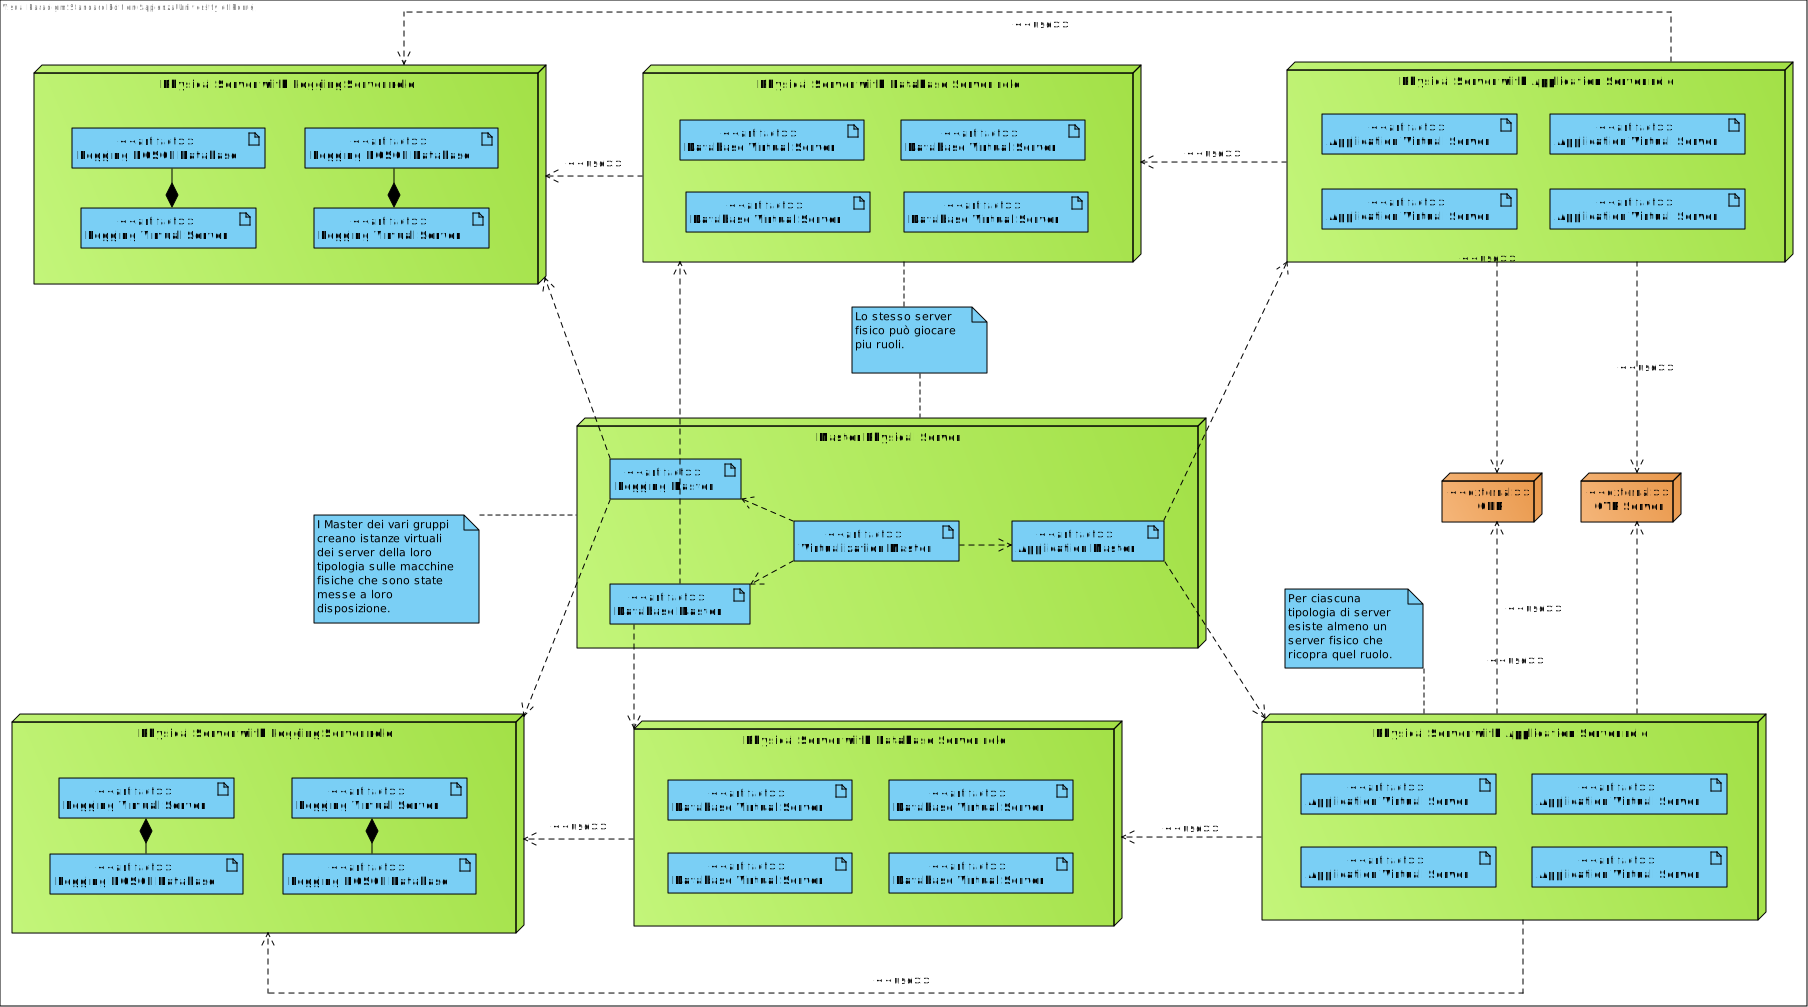
\includegraphics[width=\textheight, angle=90]{Images/Physical_View.eps}
	\caption{Diagramma di deployment del sistema.}
	\label{fig:physical-view}
\end{figure*}

I ruoli comprendono:
\begin{description}
	\item[Database Server] macchina abilitata all'esecuzione di istanze del database di HBS;

	\item[Application Server] macchina abilitata all'esecuzione di istanze dell'applicazione principale di HBS;

	\item[Logging Server] macchina abilitata all'esecuzione di istanze del sistema di logging.
\end{description}
Ciascuna macchina pu\`o ricoprire diversi ruoli.

Una macchina nel sistema ricopre il ruolo di \emph{master}.
Su questa macchina sono in esecuzione i processi di gestione delle istanze del database, dell'applicazione principale, e dei sistemi di logging.
I processi di gestione dei sotto-sistemi si occupano di avviare istanze virtuali dei propri sotto-sistemi sulle macchine messe a disposizione dal \emph{virtualization master}.

Le connessioni effettuate dai clienti della banca vengono distribuite dall'\emph{application master} alle istanze di \emph{application virtual server} con una politica di \emph{load balancing}.

Il sistema di Logging mantiene un log distribuito e non ordinato delle azioni effettuate dagli utenti in un database non relazionale.


